\setlength{\footskip}{8mm}

\chapter{METHODOLOGY}

A \textbf{big figure} here, explaining your whole methodology (see Figure \ref{fig:sourcetasktraining} for example).

\begin{figure}[hbt!]
\caption{Overview of multi-task pre-training with prefix approach.}
\centerline{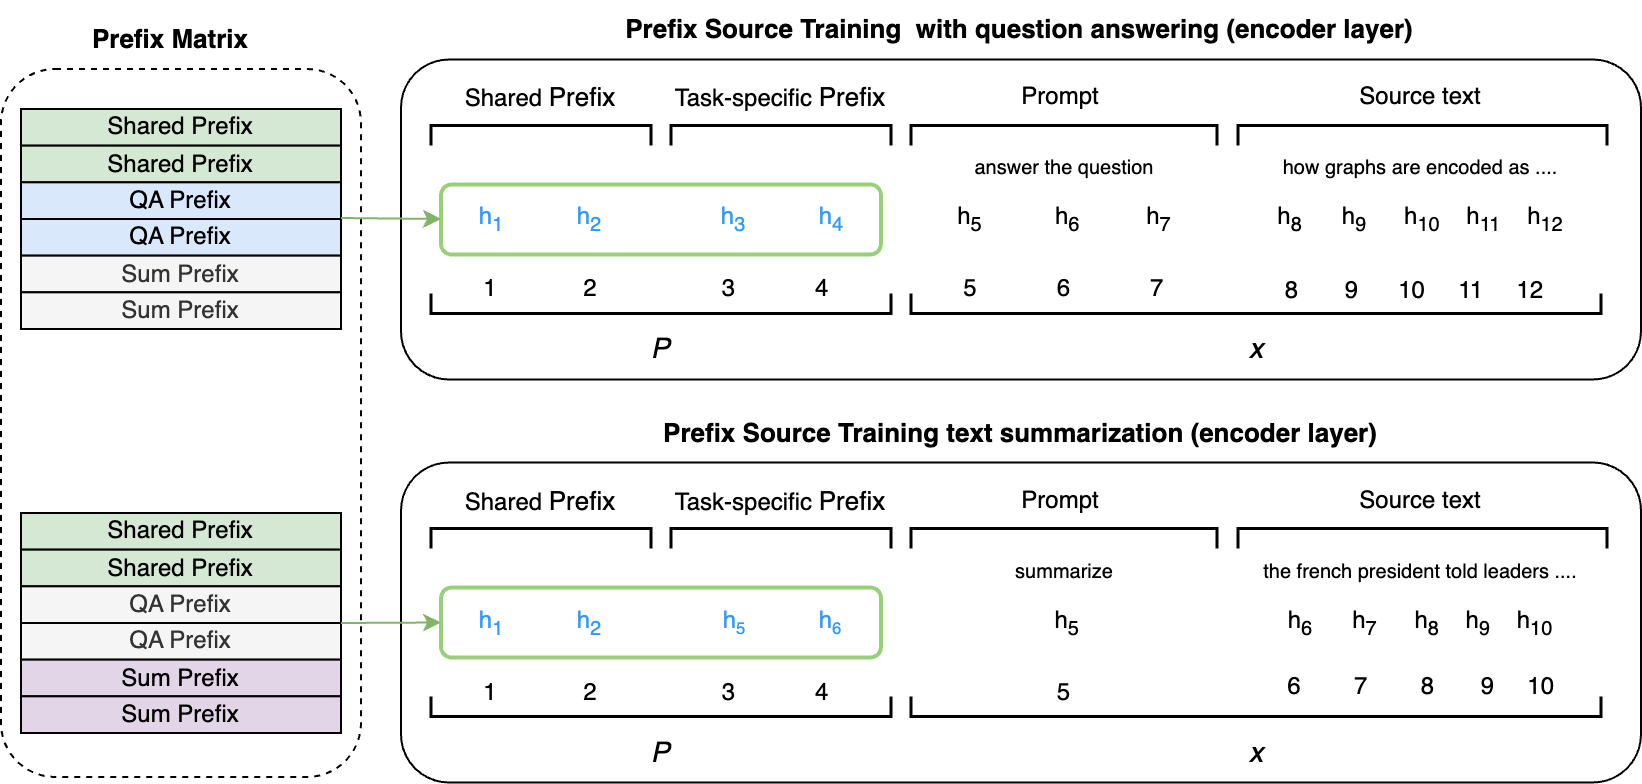
\includegraphics[width=15cm]{figures/sourcetasktraining.png}}
\label{fig:sourcetasktraining}
\small{\textit{Note.} For each task, it corresponds to different sub-prefix embeddings. Here, The prefix embedding indices for text summarization is [1, 2, 3, 4] and it changes to [1, 2, 5, 6] for QA where indices [1, 2], [3, 4], [5, 6] correspond to shared-task, text summarization and question answering respectively.}
\end{figure}

\textbf{A symbol of good methodology is that people read it,  they can reproduce it.  So make sure you are very clear what you did and write it clearly.  Follow the convention in your field of study.}}

Here I cannot guide you how to write your methodology.  It basically breaks down your proposed system into components and demonstrate your algorithm or models or systems.  

If you are pure HCI user study,  then you can just copy the Experiment chapter and call it your methodology.

This is an example:
\section{Prefix Pre-Training}
In order to facilitate learning, we aim to transfer task-specific knowledge from text summarizing and question-answering (source tasks) to query-focused summarization (target task). In addition to the two source tasks, we also incorporate shared-task prefix (see Figure \ref{fig:phase1}). This is done via prefix tuning. 

\subsection{Prefix-tuning} \label{subsection-prefix-tuning}

Considering a transformer-based encoder-decoder such as Bart \cite{lewis2019bart} $LM_{\theta} = [LM_{en}; LM_{de}]$ parameterized by $\theta$, as our pretrained model, for each task $t$, we inject task-specific prefix vectors of encoder $(P_{en})$ and decoder $(P_{de})$, $P_{\theta_{p}} = [P_{en}; P_{de}]$ parameterized by $\theta_{p}$, into the model. Following \citet{li2021prefix}, the prefix vectors are prepended to each transformer layer as additional key and value vectors. Hence, we obtain $LM_{\theta, \theta_{p}} = [P_{en}; LM_{en}; P_{de}; LM_{de}]$

For the pre-training, given the input document $X$, the objective is to minimize the negative log-likelihood of generating the target output $Y = \{y_{1}, y_{1}, ..., y_{|Y|} \}$:

\begin{equation}
L(\theta , \theta_{p}) = \sum_{i}^{|Y|} log \mathbb{P}(y_{i} | X, y_{1}, ..., y_{i-1}) 
\end{equation}

Note that the prefix parameters $\theta_{p}$ are trainable while the parameters of LM $\theta$ are either kept intact or being updated. Next, we further explain how we perform 1) Multi-task Pre-Training with Prefix; and 2) Single-task Pre-Training with Prefix in details below.

% and taking the encoder layer in transformer as an example, let $z = [x]$ denote its input sequence. We use $h_{i}$ to represent the concatenation of all activation from all layers at the index $i$. The $h_{i}$ for all $i\in x$ in encoder layer is a function of $z_{i}$ and the other activations in the context based on the LM, as follows:

% \[h_{i} = LM_{\phi}(z_{i}, h_{\neq i}) \]

% Prefix-tuning prepends prefixes for the encoder layer to obtain $z = [prefix;x]$. In this case, the length of the prefix is represented by $|P_{idx}|$, while the series of prefix embedding indices is represented by $P_{idx}$. The prefix parameters are initialized to be stored in a trainable matrix $P_{\theta} \in R^{|P_{idx}| \times d}$ where $d$ is the LM dimension. During the training, only respective prefix are updated by maximizing the likelihood of generating the target sequence $y$, as follows:

% $h_{i} = \left\{\begin{matrix} P_{\theta}[i, :], &  if i \in P_{idx}\\ LM_{\phi}(z){i}, h_{\neq i}) & otherwise \end{matrix}\right.$

% During the training in prefix-tuning, the objective maintains the same as normal task, but only the prefix parameters $\theta$ are trainable and the parameters of the $LM_{\theta}$ are fixed. In this case, the prefix parameters contain all the task-specific knowledge learned from the training.


\subsection{Multi-Task Pre-Training with Prefix}
Similar to prefix-tuning, a trainable parameters $P_{\theta_{p}}$ is used to store the prefix embedding parameters. However, the difference is that there are $n$ tasks denoted as $[task_{1}, ..., task_{n}] $. Here, we denote $P_{idx}$ to represent the prefix embedding indices, and $|P_{idx}|$ is denoted as total prefix length. Hence, the trainable prefix $P_{\theta_{p}} \in |P_{idx}| \times dim_{p}$ is initialized to store the prefix parameters. 

In the multi-task setting, the matrix $P_{\theta_{p}}$ is decomposed into text summarization  $P_{\theta_{p}}^{sum} \in |P_{idx}^{sum}| \times dim_{p} $, question-answering $P_{\theta_{p}}^{qa} \in |P_{idx}^{qa}| \times dim_{p}$ and shared-task prefix $P_{\theta_{p}}^{shared} \in |P_{idx}^{shared}| \times dim_{p}$. For each task, it corresponds to different sub-prefix embeddings. Hence, prefix embedding indices for text summarization differ from those of QA. For instance, the length of task-specific prefix and shared-task prefixes are set to 2. The prefix embedding indices for text summarization is [1, 2, 3, 4] and it changes to [1, 2, 5, 6] for QA where indices [1, 2], [3, 4], [5, 6] correspond to shared-task, text summarization and question answering respectively (See Figure \ref{fig:sourcetasktraining}).

Specifically, during the training, it is optimized according to the following objective:

\begin{equation}
L(\theta , \theta_{p_{idx}^{task}}) = \sum_{i}^{|Y|} \log \mathbb{P}(y_{i} | X, y_{1}, ..., y_{i-1}) 
\end{equation}

Note that for fine-tuning pre-trained model setting, following the work of \citet{chen2023unisumm}, we set different weight decay regularization on different parameters for the prefixes and pre-trained model. Specifically, prefixes and pre-trained model have separate optimizers during pre-training where lower weight decay value $d_{p} = 0.01$ is set on prefix optimizer and a higher weight decay value $d = 0.05$ is set on pre-trained model. This enables prefixes to flexibly learn task-specific knowledge and enforces pre-trained model to learn broader generalization across different tasks. 

Formally, at training step $i$:
\begin{equation}
\theta^{i+1} = (1-d)\theta^{i} - \alpha ^{i}\bigtriangledown f^{i}(\theta^{i})
\end{equation}

\begin{equation}
\theta^{i+1}_{p} = (1-d_{p})\theta^{i}_{p} - \alpha ^{i}_{p}\bigtriangledown f^{i}_{p}(\theta^{i}_{p})
\end{equation}

where $\alpha^{i}$ and $\alpha^{i}_{p}$ are the learning rates for pretrained model and prefixes, and $\bigtriangledown f^{i}(\theta^{i})$ and $\bigtriangledown f^{i}_{p}(\theta^{i}_{p})$ are the batch gradient for pretrained model and prefix.

% Note that for the unfrozen LM setting, we optimize $\theta$ and $\theta_{p_{idx}^{task}}$  together.


% Taking encoder as an example, a trainable parameters $P_{en} \in |P_{idx}| \times  prefix \ dim$ is initialized to store the encoder prefix embedding parameters where $P_{idx}$ represents the prefix embedding indices, and $|P_{idx}|$ is denoted as total prefix length.  


% Specifically we use $P_{idx}^n$ to denote the indices of prefix embedding of $task_{n}$  

% Following the work of \cite{yuan2022few}, we decompose QS into QA and Sum and obtain shared and task specific knowledge through pre-fix tuning approach \cite{li2021prefix} from large-scale data such as SQUAD \cite{rajpurkar2016squad}, and XSUM \cite{xsum}. 
\subsection{Single-Task Pre-Training with Prefix}
In contrast to multi-task learning where matrix $P_{\theta_{p}}$ is decomposed into text summarization  $P_{\theta_{p}}^{sum} \in |P_{idx}^{sum}| \times dim_{p} $, question-answering $P_{\theta_{p}}^{qa} \in |P_{idx}^{qa}| \times dim_{p}$ and shared-task prefix $P_{\theta_{p}}^{shared} \in |P_{idx}^{shared}| \times dim_{p}$, in single-task setting, each task is independently learned. Note that for fine-tuning pre-trained model setting, the model learns together with shared-task prefix.

% \subsection{Shared-task Prefix Pre-Training}


\section{Applying the Pre-Trained Prefix to Target Task}
After training on source tasks, we obtain the prefix parameters that contain task specific knowledge from text summarization and question-answering. We continue vanilla prefix-tuning on it. Note that we can apply the trained prefixes in two manners, one with two source task and a shared-task prefix and one with only the shared-task prefix.